\RequirePackage{iftex}
\ifPDFTeX
\documentclass[a4paper,12pt]{article}
\usepackage[margin=24mm]{geometry}
\usepackage[T1]{fontenc}
\usepackage[utf8]{inputenc}
\usepackage{graphicx}
\usepackage{CJKutf8}
\else
\documentclass[a4paper,12pt]{jsarticle}
\usepackage[dvipdfmx,margin=24mm]{geometry}
\usepackage[dvipdfmx]{graphicx}
\fi
\usepackage{amsmath,amssymb,amsthm}
\usepackage{enumitem}
\usepackage{tikz}
\usepackage{url}
\usetikzlibrary{arrows.meta,calc}

\setlength{\parindent}{0pt}
\setlength{\parskip}{0.35em}
\setlength{\fboxsep}{8pt}
\setlist[itemize]{leftmargin=2em,itemsep=0.25em,topsep=0.35em}

\newcommand{\feedbackqa}[2]{%
\item[]
\begin{tabular}[t]{@{}p{1.8em}@{\hspace{0.4em}}p{\dimexpr\linewidth-2.2em\relax}@{}}
Q. & #1 \\
A. & #2
\end{tabular}
\par\smallskip\hrulefill
}

\newcommand{\pointbox}[1]{%
\begin{center}
\fbox{%
\begin{minipage}{0.9\linewidth}
#1
\end{minipage}}
\end{center}
}

\begin{document}
\ifPDFTeX
\begin{CJK}{UTF8}{min}
\fi

\theoremstyle{definition}
\newtheorem*{definition}{定義}
\newtheorem*{theorem}{定理}
\newtheorem*{example}{例}
\newtheorem*{remark}{注意}

\begin{center}
{\LARGE 数学1A 第3回レジュメ}\\[0.4em]
微分可能性と平均値の定理
\end{center}

\section*{フィードバック}

\begin{itemize}[leftmargin=1.5em,itemsep=0.7em,topsep=0.3em]
\feedbackqa{中間試験はあるか？}{中間試験はあります。ただし、成績には$$\max\{\text{小テスト }20\%+\text{期末 }80\%,\ \text{小テスト }10\%+\text{中間 }30\%+\text{期末 }60\%\}$$のような形で反映されます（シラバスの成績の付け方を参照）。}
\feedbackqa{期末は教科書のレベルを超えるか？}{期末は教科書の内容を超えることはありませんが、難易度については教科書を超える問題もあるかもしれません。}
\feedbackqa{男女の席に隔たりがある}{せっかくなので、中間試験の前に一度グループワークでもしようかなと思います。}
\feedbackqa{証明のニコチャンマーク？}{証明の始まりと終わりで使います。証明のはじめの憂鬱な気持ちと、証明が終わったときの晴れやかな気持ちを表しています。}
\feedbackqa{中間値の定理は今後使うか？}{数学科ではよく使いますが、他学科では2年生以降はあまり使わないと思います。中間・期末では出る可能性はありますが。}
\feedbackqa{$(\log x)' = 1/x$の証明はどうやるか？}{通常は、まず$e^x$の微分を求め、$\log$が$e^x$の逆関数であることを利用して示します。大変なので授業ではやりませんが、興味があれば \url{https://hiraocafe.com/note/differential-of-logarithm.html} を参照してください。}
\feedbackqa{平均値の定理は必ず成り立つのか？ 微分後の式が曲線の場合、$h$は成り立たないのではないか？}{「曲線」というのはどういう意味でしょうか。グラフが関数ではなく曲線で与えられている場合はでしょうか？その場合は一般には成り立たないですが、それに対応する定理があったと思います（名前はど忘れしましたが、、）。}
\feedbackqa{高校範囲と大学範囲の違い}{この授業では、高校数学と重なる部分もかなりあると思います。高校で扱っていない内容としては、テイラーの定理と多変数関数の微分があります。}
\feedbackqa{おすすめの問題集}{教科書の章末問題は基本的な問題が多いですし、慶應義塾大学の先生が作っているので、期末テストなどの対策にもよいかと思います。} 
\feedbackqa{教科書がわかりにくい}{おっしゃるとおりだと思います。責任の一端を感じます。}
\feedbackqa{物理では$\dot{f}$を微分として使う}{慣習の違いだと思います。物理では時間微分を表すのにドットを使うことが多いですね。どちらを使っていただいても構いません。数学では$f'$を使うので、そのまま使っています。}
\feedbackqa{定理とついているものは自明に使ってよいか？}{使ってよいですが、使ったときはどの定理を使ったか書くようにしましょう。}
\feedbackqa{$\epsilon$-$N$をやる予定はあるか？}{今のところありません。要望があればやるかもしれません。}
\feedbackqa{難しい分野が出るのはいつからか？}{この授業ではそんなに難しい分野は出てきませんが、来週以降に出てくるテイラー展開は、初めて見たときにはぎょっとすると思います。}
\feedbackqa{定理の証明があいまい}{そのとおりですし、そこに気がつくのはよいことだと思います。厳密にやろうと思うと時間がかかるので、かなり端折っています。不思議に感じたことがあれば、いつでも質問してください。}
\feedbackqa{微分の公式の証明で使えるトリックを教えてほしい}{よく使うのは、「同じものを足して引く」「同じものをかけて割る」という操作です。微分の合成では、$\phi(x)-\phi(a)$をかけて割りました。}
\feedbackqa{高校数２はどこが面白い？}{正直、数2はつまらないと思っていました。}
\feedbackqa{数学のいろんな書き方で困惑している。負の実数は$x<0$と書けばよいのか？ などなど}{同じ意味を表す書き方でも、いろいろな表現があります。負の実数は、$x<0$と書いてもよいですし、$x\in \mathbb R_{-}$や$x\in (-\infty,0)$と書いても、どれでも大丈夫です。その人の趣味や分野によっても変わってきますので、慣れですかね。}
\feedbackqa{一限で眠い}{お気持ちはよくわかりますが、よい大学生活を送るうえでも、適度な早起きは大事です。}
\feedbackqa{前の黒板が人で見えない}{前に移動するしかないですね。}
\feedbackqa{新しい記号になれない。}{とりあえず、新しい記号は前回までで全部ですので、徐々に慣れていってくれたらよいです。}
\feedbackqa{誕生日だけど授業にきた。}{とても偉いですね。}
\feedbackqa{問題演習をもっとしたい}{時間がないので何とも言えませんが、なるべくやれるように努めます。}
\feedbackqa{中間値の定理は$[a,b]$上連続だったが、閉区間である必要はあるか？}{例えば、$f(0)=0$で、$x>0$では$f(x)=1$とすると、$f$は$(0,1)$上連続で、$(0,1)$上では微分可能ですが、$f(0)=0$, $f(1)=1$です。$\lambda=1/2$とすると、$f(c)=1/2$となる$c$はありません。したがって、区間の両端で連続である必要があります。}
\feedbackqa{黒板がよみにくいときがある}{ご指摘ありがとうございます。気分にも影響されるので、なるべくきれいに書くよう努めます。（添字などは小さくて読みにくいこともあると思いますが、読みにくいときはぜひ聞いてください。）}
\feedbackqa{科学実験のあとに物理演習は意地悪}{どういうことでしょうか？}
\feedbackqa{好きな漫画や小説？}{最近はあまり読んでいないですね。小説は「月は無慈悲な夜の女王」を最近読んでいます。}
  \end{itemize}

\section*{小テスト}

\subsection*{問題}

問1. 次を $\forall,\exists$ などの記号を用いて書け。
\begin{itemize}
\item $(1)$ 任意の実数 $x$ について，$x^2\geq 0$
\item $(2)$ ある正の実数 $a$ が存在して，$a+1>0$
\end{itemize}

問2. $f(x)=\log |x|$ の $x\neq 0$ における微分を計算せよ。ただし$(\log x)' = 1/x$ $(x>0)$は用いて良い.

\subsection*{解答}

問1.
\begin{itemize}
\item $(1)$ $\forall x \in \mathbb{R}, x^2 \geq 0$
\item $(2)$ $\exists a \in \mathbb{R}_{>0}, a+1>0$
\end{itemize}

問2. $x\neq 0$ とする。

$x>0$ のときは $|x|=x$ だから
\[
f(x)=\log x
\]
である。したがって仮定より
\[
f'(x)=\frac{1}{x}
\]
となる。

$x<0$ のときは $|x|=-x$ だから
\[
f(x)=\log(-x)
\]
である。ここで外側の関数を $\log u$，内側の関数を $u=-x$ とみると，合成関数の微分公式より
\[
f'(x)=\frac{1}{-x}\cdot \frac{d}{dx}(-x)
=\frac{1}{-x}\cdot (-1)
=\frac{1}{x}
\]
となる。

よって
\[
(\log|x|)'=\frac{1}{x}\qquad (x\neq 0)
\]
である。

\section*{1. 微分可能性}

\begin{definition}
関数 $f$ が点 $a$ で微分可能であるとは，極限
\[
f'(a)=\lim_{h\to 0}\frac{f(a+h)-f(a)}{h}
\]
が存在することをいう。
\end{definition}

差商
\[
\frac{f(a+h)-f(a)}{h}
\]
は，点 $(a,f(a))$ と $(a+h,f(a+h))$ を結ぶ割線の傾きである。$h\to 0$ とした極限が存在するとき，それが接線の傾き $f'(a)$ になる。

\begin{center}
\begin{tikzpicture}[x=1.15cm,y=1.15cm,>=Latex]
\pgfmathsetmacro{\xa}{1.55}
\pgfmathsetmacro{\xb}{2.65}
\pgfmathsetmacro{\fa}{0.12*(\xa-0.8)^2+0.42*\xa+0.45}
\pgfmathsetmacro{\fb}{0.12*(\xb-0.8)^2+0.42*\xb+0.45}
\pgfmathsetmacro{\ta}{0.24*(\xa-0.8)+0.42}
\draw[->] (-0.2,0) -- (4.6,0) node[below] {$x$};
\draw[->] (0,-0.2) -- (0,3.4) node[left] {$y$};
\draw[thick,domain=0.35:4.15,samples=120,smooth] plot (\x,{0.12*(\x-0.8)^2+0.42*\x+0.45});
\draw[gray,dashed] (\xa,0) -- (\xa,\fa);
\draw[gray,dashed] (\xb,0) -- (\xb,\fb);
\fill (\xa,\fa) circle (2pt);
\fill (\xb,\fb) circle (2pt);
\draw[blue,thick] (\xa,\fa) -- (\xb,\fb);
\draw[red,dashed] ({\xa-0.9},{\fa-\ta*0.9}) -- ({\xa+2.0},{\fa+\ta*2.0});
\draw (\xa,-0.18) node {$a$};
\draw (\xb,-0.18) node {$a+h$};
\draw (3.35,2.72) node[right] {$y=f(x)$};
\draw[blue] (2.9,1.52) node[right] {割線};
\draw[red] (3.08,2.02) node[right] {接線};
\end{tikzpicture}
\end{center}

\begin{example}
\[
f(x)=|x|
\]
は $x=0$ で連続だが，微分可能ではない。実際，
\[
\lim_{h\to 0+}\frac{|h|-|0|}{h}=1,\qquad
\lim_{h\to 0-}\frac{|h|-|0|}{h}=-1
\]
となり，左右で傾きが一致しない。
\end{example}

\begin{center}
\begin{tikzpicture}[x=1.15cm,y=1.15cm,>=Latex]
\draw[->] (-2.3,0) -- (2.3,0) node[below] {$x$};
\draw[->] (0,-0.2) -- (0,2.3) node[left] {$y$};
\draw[thick,domain=-2:0] plot (\x,{-\x});
\draw[thick,domain=0:2] plot (\x,{\x});
\draw[dashed,red] (-1.6,1.6) -- (0,0);
\draw[dashed,blue] (0,0) -- (1.6,1.6);
\fill (0,0) circle (2pt);
\draw (-1.45,1.85) node[red] {左の傾き $-1$};
\draw (1.4,1.85) node[blue] {右の傾き $1$};
\draw (1.4,0.8) node {$y=|x|$};
\end{tikzpicture}
\end{center}

\begin{example}
\[
f(x)=
\begin{cases}
x^2\sin\!\left(\dfrac{1}{x}\right) & (x\neq 0),\\
0 & (x=0)
\end{cases}
\]
とする。このとき $f$ は $x=0$ で微分可能で，
\[
f'(0)=\lim_{h\to 0}\frac{h^2\sin(1/h)}{h}
=\lim_{h\to 0}h\sin(1/h)=0
\]
である。一方，$x\neq 0$ では
\[
f'(x)=2x\sin\!\left(\frac{1}{x}\right)-\cos\!\left(\frac{1}{x}\right)
\]
だから，$f'$ は $x=0$ で連続ではない。微分可能だからといって，導関数が連続とは限らない。
\end{example}

\begin{center}
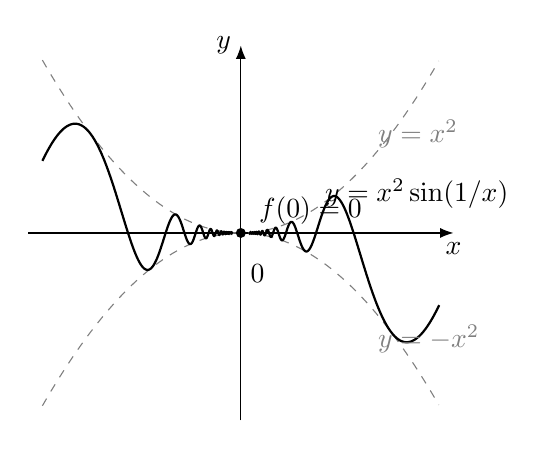
\begin{tikzpicture}[x=9cm,y=28cm,>=Latex]
\draw[->] (-0.30,0) -- (0.30,0) node[below] {$x$};
\draw[->] (0,-0.085) -- (0,0.085) node[left] {$y$};
\draw[gray,dashed,domain=-0.28:0.28,samples=120,smooth]
  plot (\x,{\x*\x});
\draw[gray,dashed,domain=-0.28:0.28,samples=120,smooth]
  plot (\x,{-(\x*\x)});
\draw[thick,domain=-0.28:-0.012,samples=1200,smooth]
  plot (\x,{\x*\x*sin((1/\x) r)});
\draw[thick,domain=0.012:0.28,samples=1200,smooth]
  plot (\x,{\x*\x*sin((1/\x) r)});
\fill (0,0) circle (1.8pt);
\draw (0,-0.010) node[below right] {$0$};
\draw[gray] (0.18,0.045) node[right] {$y=x^2$};
\draw[gray] (0.18,-0.048) node[right] {$y=-x^2$};
\draw (0.105,0.018) node[right] {$y=x^2\sin(1/x)$};
\draw (0.012,0.010) node[right] {$f(0)=0$};
\end{tikzpicture}
\end{center}

\pointbox{
今日の見方:
\[
\text{微分可能} \Longrightarrow \text{連続}
\]
だが，逆向きは一般には成り立たない。
}

\section*{2. 対数微分}

\begin{theorem}
$f$ を $f(x)\neq 0$ を満たす区間上の微分可能な関数とする。このとき
\[
\frac{d}{dx}\log|f(x)|=\frac{f'(x)}{f(x)}
\]
である。したがって
\[
f'(x)=f(x)\frac{d}{dx}\log|f(x)|
\]
が成り立つ。
\end{theorem}

\begin{proof}
合成関数の微分法より
\[
\frac{d}{dx}\log|f(x)|
=\frac{1}{f(x)}f'(x)
\]
である。両辺に $f(x)$ を掛ければよい。
\end{proof}

指数にも底にも $x$ が入る関数では，先に対数をとると計算しやすい。

\begin{example}
\[
y=x^x \qquad (x>0)
\]
を微分する。両辺の対数をとると
\[
\log y=x\log x
\]
である。したがって
\[
\frac{y'}{y}=\log x+1
\]
となるので
\[
y'=x^x(\log x+1)
\]
を得る。
\end{example}

\begin{center}
\begin{tikzpicture}[x=1.05cm,y=1.05cm,>=Latex]
\draw[->] (0,0) -- (4.8,0) node[below] {$x$};
\draw[->] (0,0) -- (0,4.2) node[left] {$y$};
\draw[thick,domain=0.45:2.2,samples=120,smooth] plot (\x,{(\x)^( \x )});
\draw[dashed] (1,0) -- (1,1);
\fill (1,1) circle (2pt);
\draw (1,-0.18) node {$1$};
\draw (-0.18,1) node {$1$};
\draw (2.5,3.5) node[right] {$y=x^x$};
\end{tikzpicture}
\end{center}

\section*{3. ロルの定理と平均値の定理}

\begin{theorem}[ロルの定理]
$f$ を $[a,b]$ で連続，$(a,b)$ で微分可能とする。さらに $f(a)=f(b)$ とする。このとき，ある $c\in (a,b)$ が存在して
\[
f'(c)=0
\]
となる。
\end{theorem}

直感的には，両端の高さが同じなら，途中のどこかで接線が水平になる。

\begin{center}
\begin{tikzpicture}[x=1.08cm,y=1.08cm,>=Latex]
\pgfmathsetmacro{\xa}{0.75}
\pgfmathsetmacro{\xc}{2.45}
\pgfmathsetmacro{\xb}{4.15}
\pgfmathsetmacro{\yab}{0.88}
\pgfmathsetmacro{\amp}{1.02}
\pgfmathsetmacro{\yc}{\yab+\amp}
\draw[->] (0,0) -- (4.7,0) node[below] {$x$};
\draw[->] (0,0) -- (0,3.3) node[left] {$y$};
\draw[thick,domain=\xa:\xb,samples=180,smooth]
  plot (\x,{\yab+\amp*(1+cos(180*(\x-\xc)/(\xb-\xc)))/2});
\draw[dashed] (0,\yab) -- (\xb,\yab);
\draw[dashed] (\xc,0) -- (\xc,\yc);
\draw[red,thick] ({\xc-0.72},\yc) -- ({\xc+0.72},\yc);
\fill (\xa,\yab) circle (2pt);
\fill (\xb,\yab) circle (2pt);
\fill (\xc,\yc) circle (2pt);
\draw (\xa,-0.18) node {$a$};
\draw (\xb,-0.18) node {$b$};
\draw (\xc,-0.18) node {$c$};
\draw (-0.08,\yab) node[left] {$f(a)=f(b)$};
\draw[red] (3.45,\yc+0.12) node[right] {$f'(c)=0$};
\end{tikzpicture}
\end{center}

\begin{theorem}[コーシーの平均値の定理]
$f,g$ を $[a,b]$ で連続，$(a,b)$ で微分可能とする。さらに $(a,b)$ の各点で $g'(x)\neq 0$ とする。このとき，ある $c\in (a,b)$ が存在して
\[
\frac{f(b)-f(a)}{g(b)-g(a)}=\frac{f'(c)}{g'(c)}
\]
が成り立つ。
\end{theorem}

\begin{proof}
\[
\phi(x)=\bigl(f(b)-f(a)\bigr)\bigl(g(x)-g(a)\bigr)
-\bigl(g(b)-g(a)\bigr)\bigl(f(x)-f(a)\bigr)
\]
とおくと，$\phi(a)=\phi(b)=0$ である。したがってロルの定理により，ある $c\in(a,b)$ が存在して $\phi'(c)=0$ となる。

微分すると
\[
\bigl(f(b)-f(a)\bigr)g'(c)-\bigl(g(b)-g(a)\bigr)f'(c)=0
\]
だから
\[
\frac{f(b)-f(a)}{g(b)-g(a)}=\frac{f'(c)}{g'(c)}
\]
を得る。
\end{proof}

\begin{remark}
$g(x)=x$ とおくと，コーシーの平均値の定理は通常の平均値の定理になる。
\end{remark}

\section*{4. ロピタルの定理}

\begin{theorem}
$f,g$ を $a$ の近くで微分可能とし，$f(a)=g(a)=0$ とする。さらに $g'(x)\neq 0$ が成り立ち，
\[
\lim_{x\to a}\frac{f'(x)}{g'(x)}
\]
が存在するとする。このとき
\[
\lim_{x\to a}\frac{f(x)}{g(x)}
=\lim_{x\to a}\frac{f'(x)}{g'(x)}
\]
が成り立つ。
\end{theorem}

\begin{proof}
$x\neq a$ で $a$ に十分近い点をとる。区間 $[a,x]$ または $[x,a]$ にコーシーの平均値の定理を適用すると，その間のある点 $c$ について
\[
\frac{f(x)-f(a)}{g(x)-g(a)}=\frac{f'(c)}{g'(c)}
\]
となる。ここで $f(a)=g(a)=0$ だから
\[
\frac{f(x)}{g(x)}=\frac{f'(c)}{g'(c)}
\]
である。$x\to a$ とすると $c\to a$ なので，右辺は仮定した極限に収束する。よって左辺も同じ極限に収束する。
\end{proof}

\begin{example}
\[
\lim_{x\to 0}\frac{e^x-1}{x}
\]
を考える。分子も分母も $x\to 0$ で $0$ に近づくので，ロピタルの定理より
\[
\lim_{x\to 0}\frac{e^x-1}{x}
=\lim_{x\to 0}\frac{e^x}{1}=1
\]
となる。
\end{example}

\ifPDFTeX
\end{CJK}
\fi

\end{document}
